\documentclass[12pt,a4paper]{article}
\usepackage[affil-it]{authblk}
\usepackage[utf8]{inputenc}

\usepackage{ragged2e}
\justifying

% Adjusting margins to personal my need
%\addtolength{\oddsidemargin}{-.5in}
%\addtolength{\evensidemargin}{-.5in}
%\addtolength{\textwidth}{1in}
%\addtolength{\topmargin}{-.5in}
%\addtolength{\textheight}{1in}


% Graphics
\usepackage{caption}
\usepackage{subcaption}
\usepackage{graphicx}
\graphicspath{{img/}}

% Math
\usepackage{amssymb}
\usepackage{amsmath} % Required for some math elements

% Other
\usepackage{algorithmic}
\usepackage{array}
\usepackage{lipsum}
\usepackage{hyperref}



\begin{document}
\title{Spambase \\
\Large{Report per l'Esame di Fondameti di Machine Learning}
} % Title

\author{\textsc{Marco Moroni} \\
    \emph{129056} \\
    Ingegneria informatica\\
    \emph{255699@studenti.unimore.it}
  }

\date{Giugno 2021}

\maketitle
\clearpage
\begin{abstract}
\normalsize
In questo progetto si andrà a trattare ed analizzare il problema delle email spam che oggigiorno è sempre più diffuso e nocivo, soprattutto per le grandi aziende. Grazie al dataset fornito e alle dovute analisi compiute su di esso si è riuscito a catalogare le email e predirre in modo pressochè perfetto la natura di una mail (veritiera o spam).
\end{abstract}

\clearpage
\section{Introduzione}
Con Spam si intende l’invio o la ricezione di messaggi pubblicitari di posta elettronica che non sono stati richiesti e che l’utente che li riceve non ha autorizzato il mittente ad inviare.
\hfill \break \break
Obiettivo degli spammer è la pubblicità: comuni offerte commerciali, proposte di vendita di materiale pornografico o illegale, farmaci senza prescrizione medica. Il loro scopo è quello di carpire dati personali, login e password di utenti, numeri di carte di credito e di conto corrente ecc…
\hfill \break \break
Gli spammer sono, a tutti gli effetti, dei criminali. Ad esempio quelli che inviano mail simili alla famosa truffa “alla nigeriana” dove una persona che non conosci ti chiede aiuto per sbloccare enormi  quantità di denaro e ti propone di dividere parte di quel denaro, ma ti chiede, per fare questa operazione, una serie di dati bancari che sono il vero e unico obiettivo della mail.
\hfill \break \break
Lo Spam è anche strumento di truffa, ti propone improbabili progetti finanziari, cerca di farti credere che hai fatto una favolosa vincita di denaro o sei stato designato erede di grandi fortune e per mandarti questo fiume di denaro chiede  le credenziali di accesso al tuo conto corrente online.
\hfill \break \break
Gli spammers inviano le mail pubblicitarie o truffaldine a migliaia di indirizzi, questi indirizzi sono raccolti in rete in molteplici modi:
\begin{itemize}
    \item automaticamente indirizzi mail da Pagine personali, Blog, Forum o Newsgroup
\end{itemize}
\begin{itemize}
    \item Usano appositi software che costruiscono gli indirizzi di mail usando nomi e cognomi comuni
\end{itemize}
\begin{itemize}
    \item Pubblicano falsi siti web che catturano il tuo indirizzo, promettendo vantaggi e offerte mirabolanti
\end{itemize}
\begin{itemize}
    \item Acquistano indirizzi mail da altri spammers
\end{itemize}

Sorgono sempre più spesso notizie di grandi aziende, che per colpa di un dipendente non abbastanza istruito sul comportamento coretto da adottare di fronte ad una email non sicura, si ritrovano a dover sborsare migliaia di dollari, da pagare in cryptovalute, difficili quindi da tracciare.
\hfill \break
Motivo per il quale negli ultimi anni sempre più persone si stanno istruendo, e stanno istruendo gli altri sull'identificare 'a vista d'occhio' una mail spam, o comunque una mail sospetta.
\break
I vari servizi anti-spam che mettono a disposizione i diversi provider di mail (come Gmail, Outlook, Protonmail, Tutanota, Yahoo,...) il più delle volte non sono sufficienti a fermare i criminali che si nascondono dietro una banalissima ed innoqua email inviata dal 'cuggino di 4º grado che abita alle isole mauritius'.

\clearpage
\section{EDA - Analisi dei dati}
In statistica, l'analisi esplorativa del dati è un approccio di analisi del set di dati per riassumere le loro caratteristiche principali, spesso usando grafici statistici e altri metodi di visualizzazione dei dati. Un modello statistico può essere usato o meno, ma principalmente l'EDA serve a vedere cosa i dati possono dirci al di là della modellazione formale o del test di ipotesi. L'EDA è diversa dall'analisi iniziale dei dati (IDA), che si concentra più strettamente sulla verifica delle ipotesi richieste per l'adattamento del modello e la verifica delle ipotesi, e sulla gestione dei valori mancanti e sulle trasformazioni delle variabili secondo necessità.

\subsection{Strumenti utilizzati}
Per questo lavoro ho trovato necessario l'utilizzo di alcune librerie, fondamentali per l'analisi dei dati e per semplificare il lavoro dell'analista:
\begin{itemize}
    \item \textbf{pandas}: potente e veloce libreria open-source nata per analizzare e manipolare i dati in input, il suo nome deriva dal gioco di parole "python data analysis";
\end{itemize}

\begin{itemize}
    \item \textbf{pyplot}: sottolibreria open-source di matpolotlib che rende possibile la creazione di grafici, figure e linee, e permette inoltre di poter cambiare colori, forma e dimensioni.
\end{itemize}

\begin{itemize}
    \item \textbf{numpy}: libreria open-source basata su python e c++ fondamentale per lavorare con array di grandi dimensioni. A differenza delle liste di python, numpy salva i dati in memoria in maniera contigua, l'accesso, incrementando notevolmente le performance, stimate al 5000\%;
    \begin{figure}[h]
        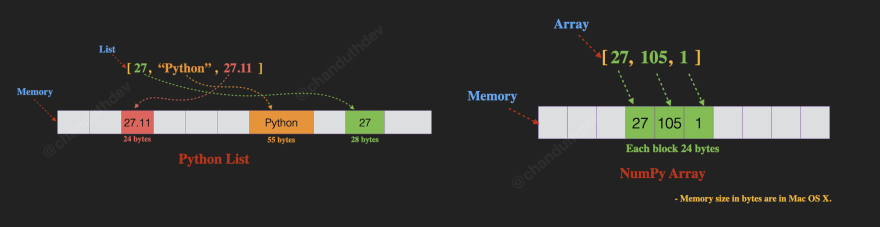
\includegraphics[width=1\columnwidth]{numpy_vs_list.png}
        \caption{}
    \end{figure}

\end{itemize}

\clearpage
\subsection{Analisi inziale}
Per prima cosa è necessario capire con che tipo di dati si andrà a lavorare, che siano numeri interi o decimali, stringhe o booleani, è fondamentale saperlo prima di cominciare l'analisi.
Per fare ciò la libreria \textit{pandas} viene in supporto fornendo delle semplici funzioni ad-hoc, come\textbf{ \textit{pandas.info()}} che permette di ricavare il numero totale di righe e colonne, e per ogni attributo, specifica il tipo di dato della colonna.
\begin{figure}[h]
    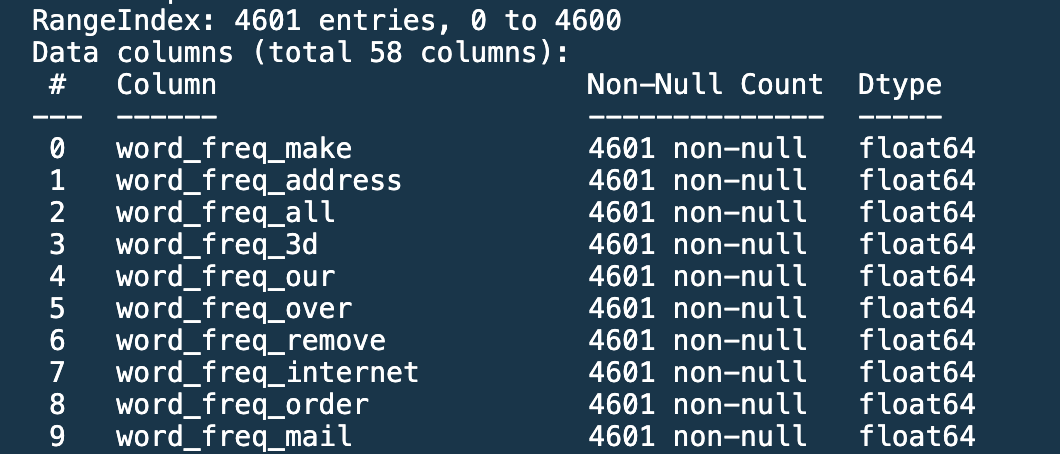
\includegraphics[width=1\columnwidth]{pandas_info.png}
    \caption{}
\end{figure}
Un'altra funzione utile è \textit{\textbf{pandas.describe()}} che per ogni colonna permette di ricavare dati come il numero di istanze non nulle, la media, la deviazione standard, il massimo e il minimo.

\begin{figure}[h]
    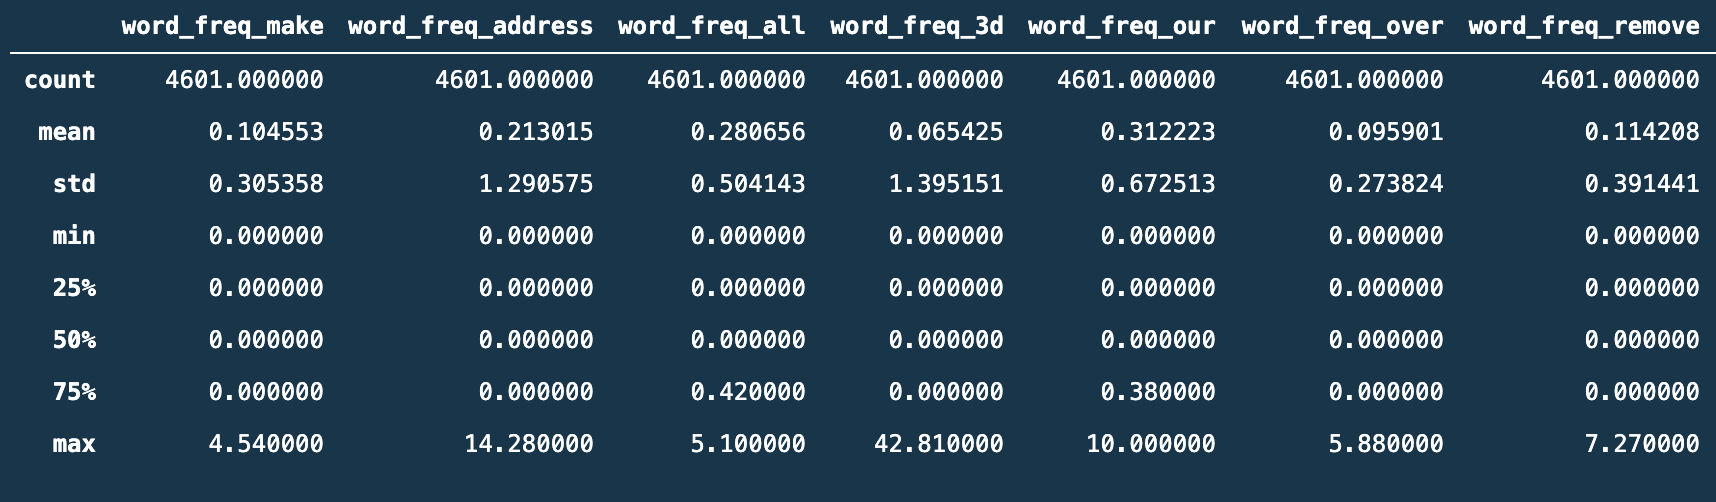
\includegraphics[width=1\columnwidth]{pandas_describe.png}
    \caption{}
\end{figure}

\subsection{Correlazione}
La matrice di correlazione è una tabella che mostra come gli attributi  siano effettivamente legati tra loro. Quando due attributi sono tra di loro correlati, al crescere dell’uno cresce anche l’altro.

Il coefficiente di correlazione è un numero, compreso tra -1 e + 1 che esprime il grado di dipendenza tra due attributi, ed in base al valore che assume si può dedurre che se il coefficente è:

\begin{itemize}
\item == 1: i due attributi hanno la stessa curva, al crescere dell'uno cresce anche l'altro;
\item == -1: i due attributi sono perfettamente decorrelati con una curva inversamente proporzionale, al crescere del primo il secondo decresce;
\item == 0: i due attributi sono indipendenti l'uno dall'altro.
\end{itemize}
 Si può notare dal grafico (fig.4) che la diagonale è composta da tutti 1, dato che un attributo messo in relazione con se stesso seguirà la stessa curva.

\begin{figure}[h]
    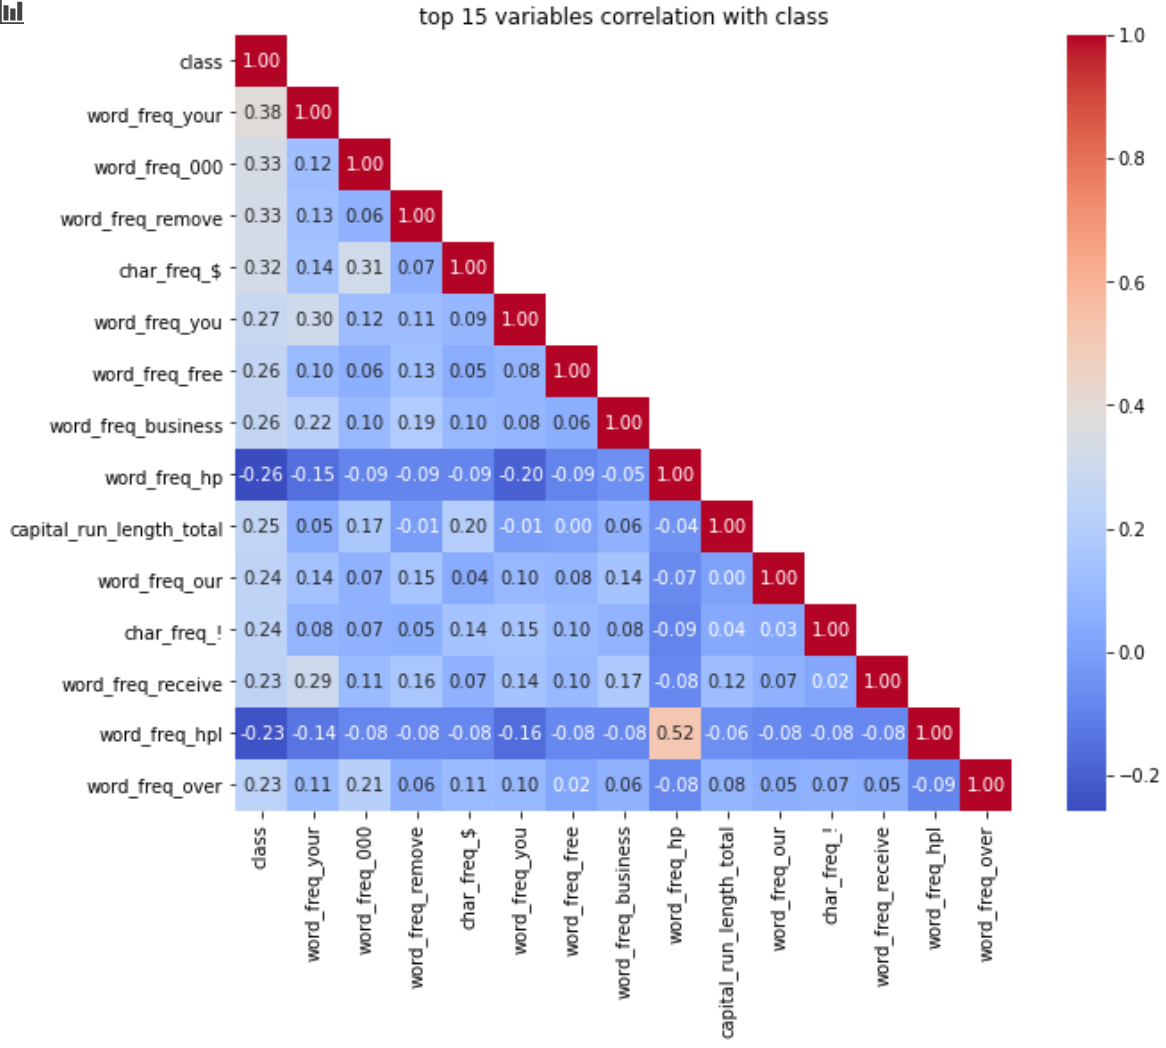
\includegraphics[width=1\columnwidth]{correlation_top_15.png}
    \caption{}
\end{figure}

Il grafico di correlazione (fig. 4) riesce a mettere in evidenza gli attributi più collegati con la classe (spam o non spam). In ordine, si notano le parole "your", "0000", "remove", "\$", "you", "free", "business", "hp", "capital\_run\_lenght\_total" (numero di lettere maiuscole), "our", "!", "receive", "hpl", "over".

Raffigurati ci sono i primi 15 attributi più collegati alla classe spam, anche se non si nota una stretta coerelazione, dato che i valori si muovono tra 0.23 e 0.38.

Si va quindi a restringere il campo per analizzare, sempre graficamente, la corrispondenza tra i cinque attributi più correlati. Si denota facilmente che la parola "your" è più presente nelle email non spam, mentre le parole "000", "remove", "\$" e "you" sono nettamente più frequenti nelle email spam.

\begin{figure}[h]
    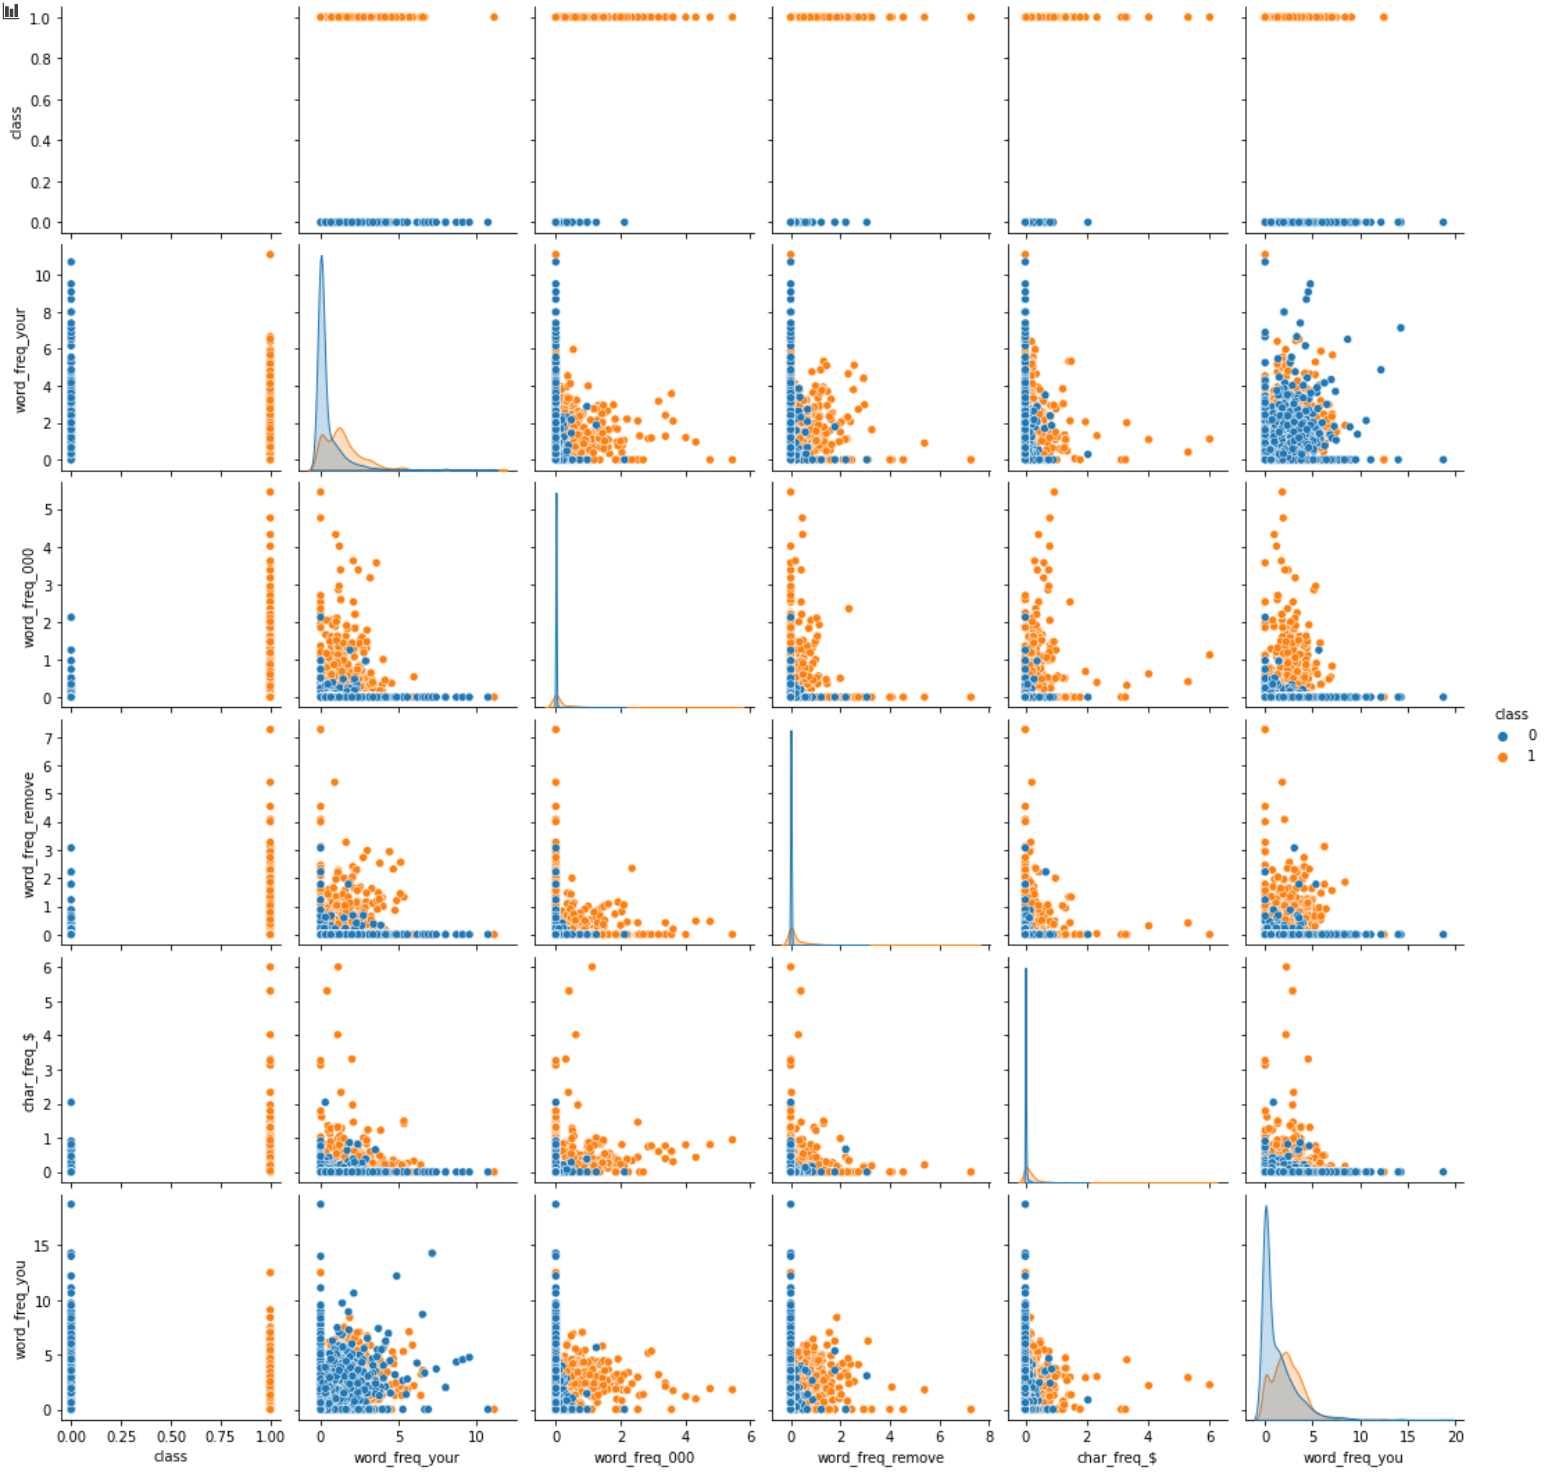
\includegraphics[width=1\columnwidth]{correlation_pair_top_6.png}
    \caption{}
\end{figure}

\subsection{Comparazione parole}
In questa sezione si andranno ad analizzare quali saranno le parole effettive da tenere maggiormente in considerazione tramite 3 grafici esplicativi.


Il grafico in figura 6 rappresenta la percentuale della frequenza di ogni singola parola trovata nelle email che sono state poi selezionate come spam. In questo grafico non si tiene conto dell'influenza delle email non spam. Il grafico conferma le analisi svolte nei capitoli precedenti, questa volta calcolando solo l'impatto delle email non spam. Le due parole più inserite sono sempre "you" e "your".


\begin{figure}[h]
    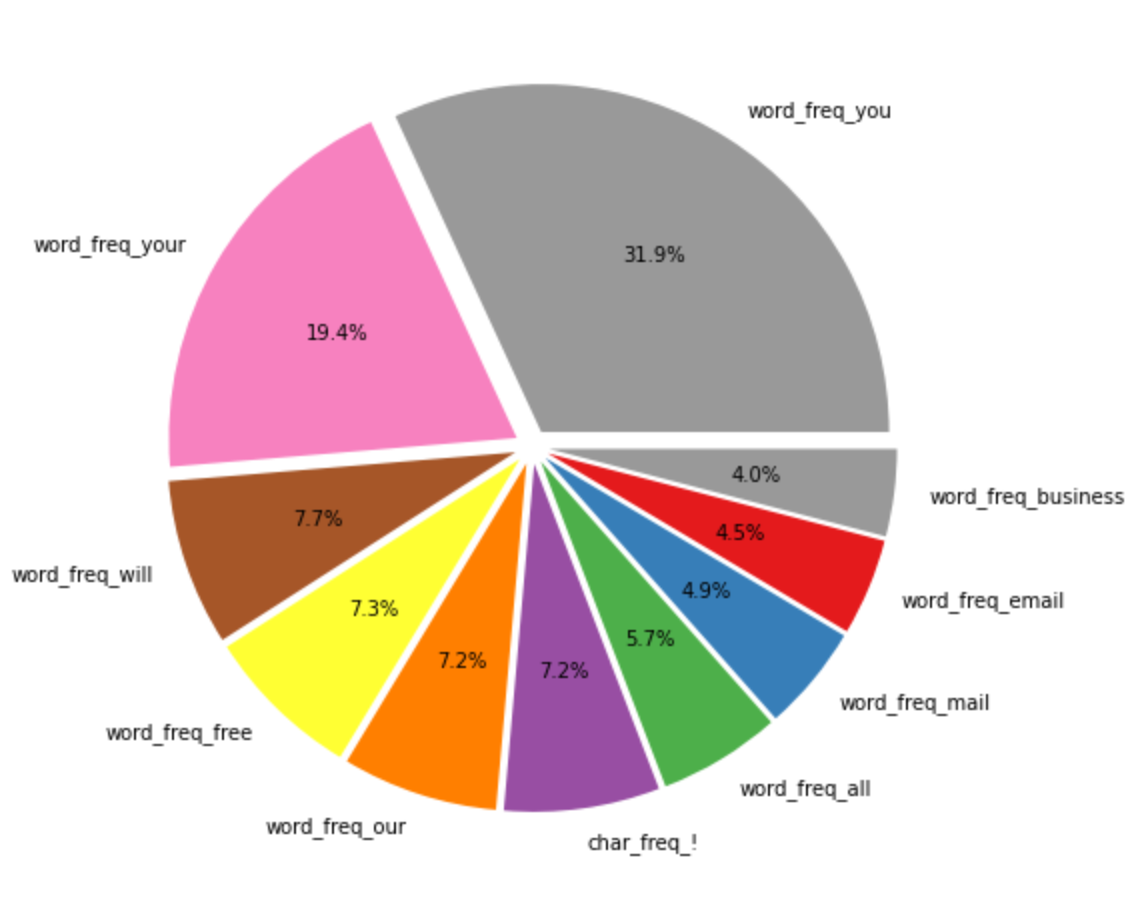
\includegraphics[width=1\columnwidth]{top_10_only_spam.png}
    \caption{}
\end{figure}
\clearpage
Per eseguire un'analisi più scrupolosa si va invece a calcolare la differenza delle frequenze tra le email non spam e le email spam.
Per fare ciò è prima necessario creare una tabella pivot che calcoli, per entrambe le classi, la media di attributo, restituendo una tabella (fig. 7) che abbia sulle ascisse le parole chiave e sulle ordinate la classe di appartenenza; i valori corrispondenti saranno la media delle frequenze della parola X nella classe di appartenenza Y.
\begin{figure}[h]
    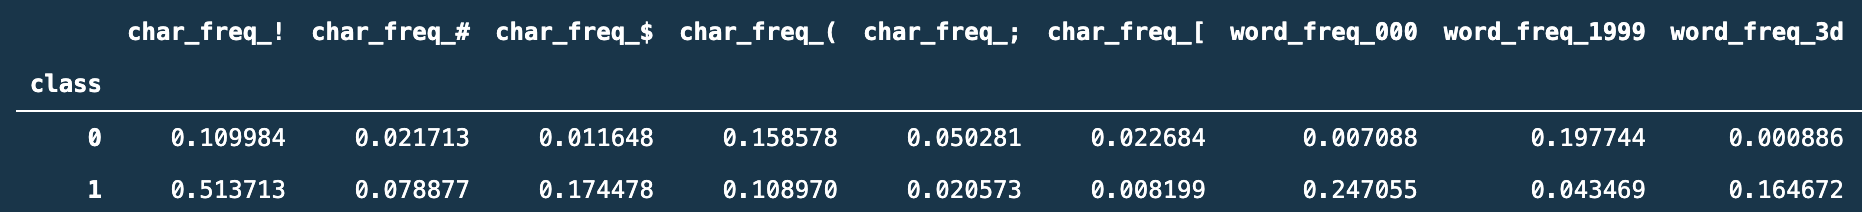
\includegraphics[width=1\columnwidth]{pivot.png}
    \caption{}
\end{figure}
Una volta calcolata la tabella pivot si notano immediatamente, dal grafico in figura 8, le parole che hanno un maggiore impatto sulla scelta della classe di appartenenza. In base al valore che ogni barra assume sulle y si determina che se:
\begin{itemize}
    \item y == 0: la parola è equamente presente sia nelle email spam che non spam;
    \item y \textless  \! 0: la parola è maggiormente presente nelle email spam;
    \item y \textgreater \!  0: la parola è maggiormente presente nelle email non spam.
\end{itemize}

\begin{figure}[h]
    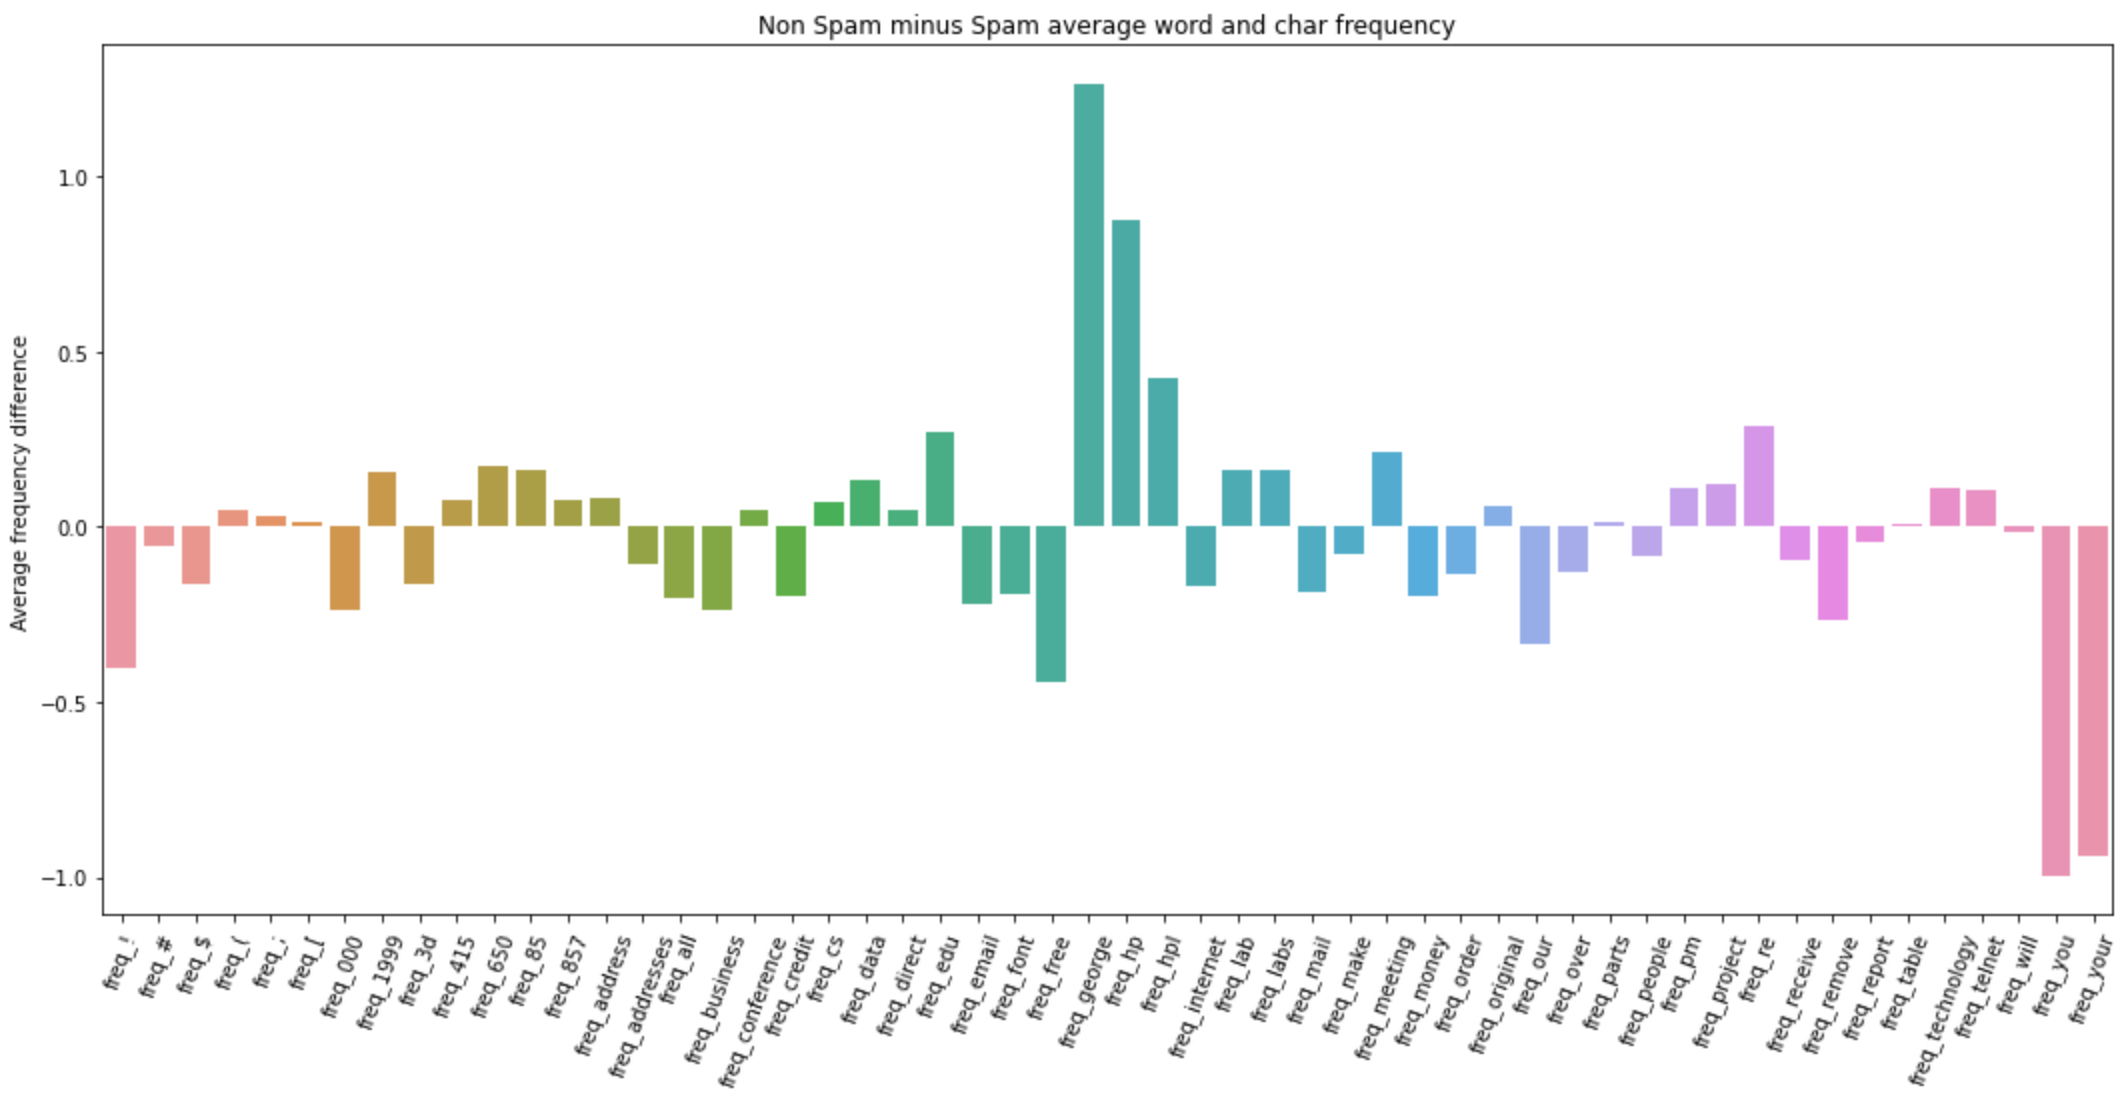
\includegraphics[width=1\columnwidth]{df_difference_barplot.png}
    \caption{}
\end{figure}

Spiccano all'occhio, quindi, che le parole "you" e "your" sono nettamente più frequenti nelle email spam, mentre le parole come "george" e "hp" sono maggiormente più frequenti nelle email vere. Questo perchè spesso, il malintenzionato che spedisce la mail malevola, non conosce il nome delle proprie vittime e li si rivolge a loro con il pronome "you" ("tu", in inglese), piuttosto che con il loro vero nome.
\subsection{Lettere maiuscole}
Nel dataset, oltre alla frequenza delle singole parole, sono presenti tre campi aggiuntivi:
\begin{itemize}
    \item capital\_run\_lenght\_average: indica la media delle lunghezze di ininterrote sequenze di lettere maiuscole;
    \item capital\_run\_length\_longest: indica la sequenza di lettere maiuscole più lunga;
    \item capital\_run\_length\_total: indica la somma totale delle lettere maiuscole.
\end{itemize}

Analizzando questi tre fattori presenti all'interno della email, si deduce, leggendo il grafico a figura 9 con le stesse valutazioni del grafico a figura 8, che nelle email spam è nettamente maggiore il numero di lettere maiuscole inserite nelle email spam.
Il malintenzionato preferisce, quindi, utilizzare le lettere maiuscole per carpire l'attenzione della vittima.

\begin{figure}[h]
    \centering
    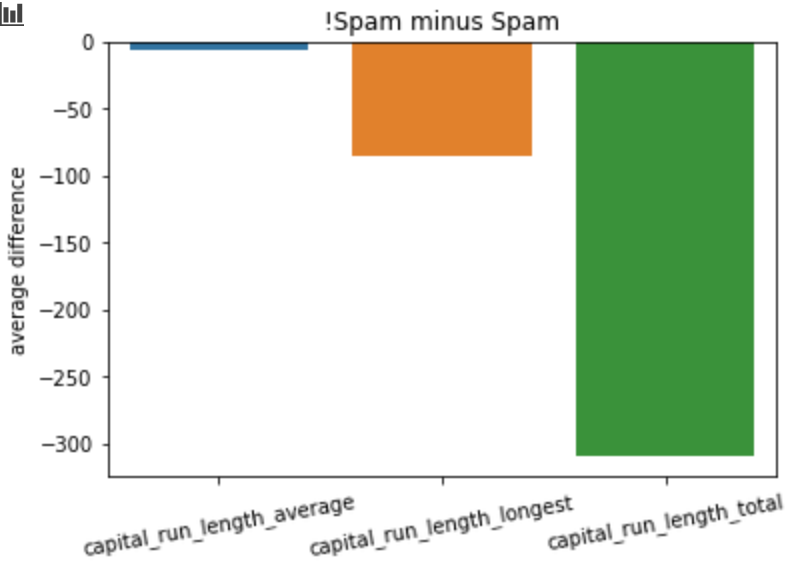
\includegraphics[scale=0.7]{capital_plot.png}
    \caption{}
\end{figure}
\section{Discussione dei modelli}
In questo capitolo si andranno a prendere come campione tre modelli per anlizzare i risultati e le performance con il dataset fornito.

\end{document}
